\documentclass[../CMPUT-404-Notes.tex]{subfiles}
\begin{document}
\chapter{HTTP}
HyperText Transport Protocol, this protocol beat FTP and Gopher because it was more flexible, extensible, and not burden with licensing agreements. 
It sends content not files which is useful if you are just searching for things and don't want to download an entire file or a small subset of that file.
Can respond to requests based on reserved VERB words like GET, POST, DELETE, PUT, etc
The flexibility comes from the fact custom headers could be included allowing for extension and adding new features.
The protocol allowed for a more request or command oriented pattern for communication. 
HTTP relied on the pairing of web clients and web servers as well as using URIs to describe resources, allowing more than 1 resources to be hosted on 1 server.
The standard for HTTP is outlined by RFC2616.

Generally HTTP uses TCP, and on port 80. For HTTPS to allow encrypted HTTP traffic using TLS it uses port 443 (generally). HTTP can work on both IPV4 and 6 addresses.
HTTP requests are made to addresses called \textbf{URIs}.

\section{HTTP Command}
Every HTTP command is made to a URI
{\centering
\begin{DndTable}[color=PhbLightGreen]{XX}
  \textbf{Command} & \textbf{What it does} \\
  GET & Retrieve information from that URI \\
  POST & Run search, log-in, append data, change data \\
  HEAD & GET without a message body (for caching) \\
  PUT & Store the entity at that URI \\
  DELETE & Delete the resource at that URI \\
  PATCH & Modify the entity at that URI \\
  OPTIONS & What options a resource can accommodate \\
  TRACE & Debugging or echo request \\
  CONNECT & Tunnelling proxy over HTTP \\
\end{DndTable}}
PATCH is not defined in RFC2616 those are in a different RFC standard.

\section{URI}
A URI is an Universal Resource Identifier, it identities i.e., points to a resource. 
Most URIs are URLs or Uniform Resource Locator but not all URLs are URIs. URLs tells you how to get to a resource. 
Some URIs are URNs or Uniform Resource Name, they tell you the unique name or number given to a resource by some body like IETF

\section{URL}
As stated before URLs or Uniform Resource Locator tells you how to get to a resource. 
It is comprised with two parts:
\begin{itemize}
  \item \textbf{Scheme} e.x., - http, https, mailto, file, data, ftp, gopher, irc, spotify
  \item \textbf{Everything else} - Anything not part of the scheme.
\end{itemize}

\subsection{URL syntax}
All URLs follow a fixed syntax

\texttt{URI = scheme:[//authority]path[?query][\#fragment]}

The authority follows another syntax listed below

\texttt{authority = [userinfo@]host[:port]}

{\centering
\begin{DndTable}[color=PhbLightGreen]{XX}
  \textbf{Syntax} & \textbf{Example} \\
  scheme & http, https \\
  authority & Can be a username and password as part of userinfo, Host followed by a port after : \\
  path & The location of the resource \\
  ? & A query string to query the resource \\
  \# & Fragments that will provide directions to a secondary resource such as a section heading within the resource \\
\end{DndTable}}

\subsection{Absolute and Relative URLs}
Both the authority and path can be absolute or relative, if the authority is missing then the authority is implied based on the current URL.
If the path has any \texttt{..} or is relative then it locates the resource based on the "current working director" of the current URL.
Examples:
\begin{itemize}
  \item Absolute authority, absolute path - http://[::1]:8000/images/web-server.svg
  \item Absolute authority, relative path - http://[::1]:8000/images/../index.html
  \item Implied authority, absolute path - /images/web-server.svg
  \item Implied authority, relative path - image/web-server.svg
\end{itemize}

\subsection{Queries}
Queries are an optional portion that can be added to a URL.
You can have one or more arguments in a key-value pair format like so \texttt{key=value\&key2=value2}.
Other separator exist like \texttt{;} instead of \texttt{\&} or just having a string and no key-value pairs.
The syntax is quite loose and it's highly dependent on the webserver. 

\subsection{Fragments}
Fragments are an optional portion that can be added to a URL.
They allow jumps to some spot in the content like a time in a video using \texttt{\#t=} in a YouTube link, or a part of a page like a section's name.

\subsection{Encodings}
Universal URIs have to be able to handle anything, including characters like spaces, accents, punctuations, emoji, etc.
For HTTP assume our URLs are Unicode UTF-8 encoded. For characters that aren't in \texttt{-.\_~0-9a-zA-Z} we use \texttt{\%} encoding.
Uses RFC 3986, space is encoded as \texttt{\%20}. For domina names we use "punycode" encoding where emojis and other special characters are converted to visible ASCII.

\section{HTTP 2}
Released in 2015, it is based on the SPDY protocol by Google and it was designed to reduce latency. 
It only supported over TLS so only on HTTPS connections and is backwards compatible with HTTP version 1's methods, including their status codes, headers, and URIs.
Instead of encoding everything as ASCII, the entire protocol communicates in binary to reduce bandwidth. 
Features that make it faster, and more responsive (lower latency) is:
\begin{itemize}
  \item \textbf{Pipelining} - Allows multiples requests to be handled at the same time instead of waiting for a response before continuing. 
  \item \textbf{Push} - Allow the servers to look into the future and sends clients content before they even request it 
  \item \textbf{Multiplexing} - Allows different types of requests to be send back to the client at the same time via interleaving.
\end{itemize}

This avoids using multiple TCP connection to a single server thus reducing the number of high-latency TCP and TLS handshakes.
Both request and response is happening at the same time and data is interleaved. Requests and responses can be prioritized.

\newpage
\section{HTTP Request}
To send a message to a \textbf{server} \emph{from} the \textbf{client} one would need to send a HTTP Request message.

\begin{Definition}{HTTP Request}
This is the grammar for a HTTP request.
\begin{verbatim}
Request = Request-Line              
         *(( general-header        
          | request-header         
          | entity-header )"\r\n")  
         "\r\n"
         [ message-body ]          
\end{verbatim}
Where: 
\begin{verbatim}
Request-Line = Method URI HTTP-Version"\r\n"  
\end{verbatim}
The request line always come first where the \texttt{Method} is the type of request, the \texttt{URI} is the "URL" and the \texttt{HTTP-Version} is what version of HTTP you are running.
For format for \texttt{HTTP-Version} is \texttt{HTTP/X.Y} where \texttt{X} is the major and \texttt{Y} is the minor version numbers.
For this project it's entire in HTTP1.1 so \texttt{HTTP-Version} should be \texttt{HTTP/1.1}.

There must be an empty line with a \texttt{CRLF} right after the header to separate the header and the body of the message.
\end{Definition}

\section{HTTP Response}
To receive a message from the server or responding to a request from the server-side one would need to send a HTTP Response message.
\begin{Definition}
{HTTP Response}
This is the grammar for a HTTP response.
\begin{verbatim}
Response = Status-Line
           *(( general-header
            | response-header 
            | entity-header )"\r\n")
           "\r\n"
           [ message-body ]
\end{verbatim}
Where:
\begin{verbatim}
Status-Line = HTTP-Version Status-Code 
Reason-Phrase"\r\n"
\end{verbatim}
Like in HTTP Request the status line comes first where the \texttt{Status-Code} is the response code and the \texttt{Reason-Phrase} is the phrase associated with the \texttt{Status-Code}.
The format is for the HTTP-Version is the same as in HTTP Request.
\end{Definition}

\section{HTTP Headers}
There are a lot of different headers that can make up a HTTP message but for all headers they follow a specific syntax
\begin{verbatim}
header = field-name":" [ field-value ]
\end{verbatim}
It's encoded like a key value pair where \texttt{field-name} is the header's name and the \texttt{field-value} is the value for that header. 

\section{GET}
HTTP GET is a simple request to be sent that resource.
\begin{itemize}
  \item It might be dynamic (resource is generated when the request is received by the software on the server), this could be done by a JavaScript or a Python CGI.
  \item It might be static (just a file sitting on the server)
  \item It might be a mix of static and dynamic content.
\end{itemize}
We can send query parameters along with a HTTP GET in the URL using the \texttt{?} character.
GET request \textbf{SHOULD NOT} cause the server to change data-we should use a different HTTP method for that. 
GET request are only used for reading data/information.
\begin{Note}
  You \textbf{SHOULD NOT} send a body with a GET Request because it might lead to a rejection. The behaviour is undefined so to keep everything working smoothly for all platforms you shouldn't send one.
\end{Note}

\subsection{Request Headers}
With HTTP 1.1 you \textbf{must} send a \texttt{Host} header with the authority you are connecting with as the value.
You \textbf{should} also send these headers as well
\begin{itemize}
  \item Connection: Keeps the connection open or not after the current transaction finishes.
  \item Date: The date of the request.
  \item Accept: Advertises which content type, expressed as MIME types the client is able to understand.
\end{itemize}


\section{POST}
HTTP POST is a request to update, create, or generally interact with a URL. 
\begin{itemize}
  \item Can do things like queries like HTTP GET but not limited by length.
  \item Use to submit HTML forms.
  \item POST is expected to add or mutate data.
\end{itemize}

Moreover POST:
\begin{itemize}
  \item URI identities a service/handler/script/process
  \item Arguments are stored in the HTTP request body
  \item The request body is interpreted by some software and processed
  \item "Send this here for processing" basically
\end{itemize}

POST can be used for:
\begin{itemize}
  \item Login/logout
  \item Reply
  \item Post on a forum/blog
  \item Upload multiple files (Somewhere)
  \item Make an order
  \item Fill out a survey/poll
\end{itemize}

\subsection{Forms}
POST methods often send their parameters in the body of the POST requests. The \texttt{Content-Type} of the body is usually some type of form
\begin{itemize}
  \item \texttt{applicaiton/x-www-form-urlencoded}
  \item \texttt{multipart/form-data} - Generally used when uploading files
\end{itemize}

Each form element has a \texttt{name}.
The \texttt{name} is the identifier used for the variable that is going to store the content.
Example: \texttt{<input name="occupation">} becomes \texttt{occupation=}
The content of the input element becomes the value.

\begin{figure}[htpb]
  \centering
  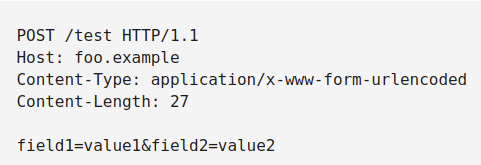
\includegraphics[width=0.8\columnwidth]{../assets/x-www-form-urlencoded.png}
  \caption{Example \texttt{x-www-form-urlencoded}}
  \label{fig:assets-x-www-form-urlencoded-png}
  https://developer.mozilla.org/en-US/docs/Web/HTTP/Methods/POST
\end{figure}


multipart/form-data uses mime (multipurpose internet mail extensions) to send form data.
Mostly used to upload files as binary, but it can be used for any form. 
Send the content-size first and then ask the server i that's okay.
The server must response with a \texttt{100 Continue} code if it can handle that size of data.
Then the client will send the body.
This interaction is a bit slower because it adds a round trip latency for confirmation with the header before sending the body.
But the confirmation is done to ensure that the client doesn't send a file that is too big for the server to handle or of a type it can't handle, etc.

\begin{figure}[htpb]
  \centering
  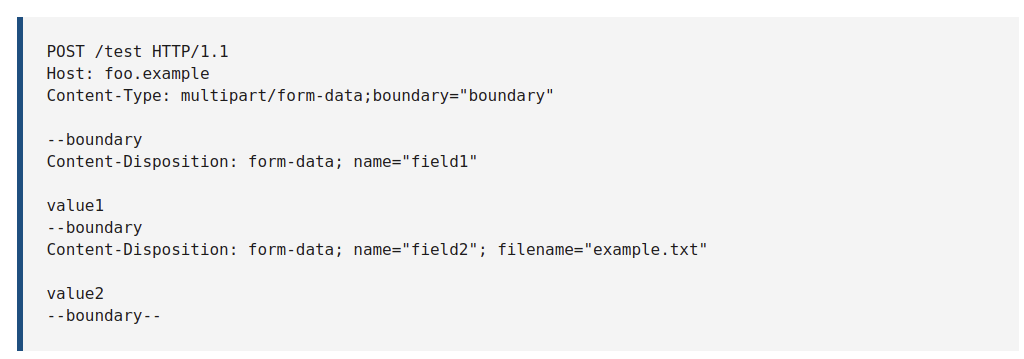
\includegraphics[width=0.8\columnwidth]{../assets/multipart-form-data.png}
  \caption{Example \texttt{mutlipart/form-data}}
  \label{fig:-assets-multipart-form-data-png}
  https://developer.mozilla.org/en-US/docs/Web/HTTP/Methods/POST
\end{figure}

The boundary lets the server tell when one part of the form ends and another begins. 
The random number should be chosen so that it won't show up in the content.
The last boundary line \textbf{must} end with \texttt{--} to tell the server that all of the form has been sent.

\subsection{Request Headers}
With HTTP 1.1 you \textbf{must} send these headers
\begin{itemize}
  \item Host: Specifies the host and port to which the request is being sent to.
  \item Content-Type: The type of the form or what type of the body.
  \item Content-Length: The size of the body.
\end{itemize}

You \textbf{should} also send these headers as well
\begin{itemize}
  \item Connection: Keeps the connection open or not after the current transaction finishes.
  \item Date: The date of the request.
  \item Accept: Advertises which content type, expressed as MIME types the client is able to understand.
\end{itemize}

\end{document}
